\documentclass[a4paper]{article}
\usepackage{lmodern}
\usepackage{amssymb,amsmath}
\usepackage{ifxetex,ifluatex}
\usepackage{fixltx2e} % provides \textsubscript
\ifnum 0\ifxetex 1\fi\ifluatex 1\fi=0 % if pdftex
  \usepackage[T1]{fontenc}
  \usepackage[utf8]{inputenc}
\else % if luatex or xelatex
  \ifxetex
    \usepackage{mathspec}
  \else
    \usepackage{fontspec}
  \fi
  \defaultfontfeatures{Ligatures=TeX,Scale=MatchLowercase}
    \setmainfont[]{NanumGothic}
\fi
% use upquote if available, for straight quotes in verbatim environments
\IfFileExists{upquote.sty}{\usepackage{upquote}}{}
% use microtype if available
\IfFileExists{microtype.sty}{%
\usepackage{microtype}
\UseMicrotypeSet[protrusion]{basicmath} % disable protrusion for tt fonts
}{}
\usepackage[margin=1in]{geometry}
\usepackage{hyperref}
\hypersetup{unicode=true,
            pdftitle={class Project 1},
            pdfauthor={Learning Spoons},
            pdfborder={0 0 0},
            breaklinks=true}
\urlstyle{same}  % don't use monospace font for urls
\usepackage{color}
\usepackage{fancyvrb}
\newcommand{\VerbBar}{|}
\newcommand{\VERB}{\Verb[commandchars=\\\{\}]}
\DefineVerbatimEnvironment{Highlighting}{Verbatim}{commandchars=\\\{\}}
% Add ',fontsize=\small' for more characters per line
\newenvironment{Shaded}{}{}
\newcommand{\KeywordTok}[1]{\textcolor[rgb]{0.00,0.00,1.00}{#1}}
\newcommand{\DataTypeTok}[1]{#1}
\newcommand{\DecValTok}[1]{#1}
\newcommand{\BaseNTok}[1]{#1}
\newcommand{\FloatTok}[1]{#1}
\newcommand{\ConstantTok}[1]{#1}
\newcommand{\CharTok}[1]{\textcolor[rgb]{0.00,0.50,0.50}{#1}}
\newcommand{\SpecialCharTok}[1]{\textcolor[rgb]{0.00,0.50,0.50}{#1}}
\newcommand{\StringTok}[1]{\textcolor[rgb]{0.00,0.50,0.50}{#1}}
\newcommand{\VerbatimStringTok}[1]{\textcolor[rgb]{0.00,0.50,0.50}{#1}}
\newcommand{\SpecialStringTok}[1]{\textcolor[rgb]{0.00,0.50,0.50}{#1}}
\newcommand{\ImportTok}[1]{#1}
\newcommand{\CommentTok}[1]{\textcolor[rgb]{0.00,0.50,0.00}{#1}}
\newcommand{\DocumentationTok}[1]{\textcolor[rgb]{0.00,0.50,0.00}{#1}}
\newcommand{\AnnotationTok}[1]{\textcolor[rgb]{0.00,0.50,0.00}{#1}}
\newcommand{\CommentVarTok}[1]{\textcolor[rgb]{0.00,0.50,0.00}{#1}}
\newcommand{\OtherTok}[1]{\textcolor[rgb]{1.00,0.25,0.00}{#1}}
\newcommand{\FunctionTok}[1]{#1}
\newcommand{\VariableTok}[1]{#1}
\newcommand{\ControlFlowTok}[1]{\textcolor[rgb]{0.00,0.00,1.00}{#1}}
\newcommand{\OperatorTok}[1]{#1}
\newcommand{\BuiltInTok}[1]{#1}
\newcommand{\ExtensionTok}[1]{#1}
\newcommand{\PreprocessorTok}[1]{\textcolor[rgb]{1.00,0.25,0.00}{#1}}
\newcommand{\AttributeTok}[1]{#1}
\newcommand{\RegionMarkerTok}[1]{#1}
\newcommand{\InformationTok}[1]{\textcolor[rgb]{0.00,0.50,0.00}{#1}}
\newcommand{\WarningTok}[1]{\textcolor[rgb]{0.00,0.50,0.00}{\textbf{#1}}}
\newcommand{\AlertTok}[1]{\textcolor[rgb]{1.00,0.00,0.00}{#1}}
\newcommand{\ErrorTok}[1]{\textcolor[rgb]{1.00,0.00,0.00}{\textbf{#1}}}
\newcommand{\NormalTok}[1]{#1}
\usepackage{graphicx,grffile}
\makeatletter
\def\maxwidth{\ifdim\Gin@nat@width>\linewidth\linewidth\else\Gin@nat@width\fi}
\def\maxheight{\ifdim\Gin@nat@height>\textheight\textheight\else\Gin@nat@height\fi}
\makeatother
% Scale images if necessary, so that they will not overflow the page
% margins by default, and it is still possible to overwrite the defaults
% using explicit options in \includegraphics[width, height, ...]{}
\setkeys{Gin}{width=\maxwidth,height=\maxheight,keepaspectratio}
\IfFileExists{parskip.sty}{%
\usepackage{parskip}
}{% else
\setlength{\parindent}{0pt}
\setlength{\parskip}{6pt plus 2pt minus 1pt}
}
\setlength{\emergencystretch}{3em}  % prevent overfull lines
\providecommand{\tightlist}{%
  \setlength{\itemsep}{0pt}\setlength{\parskip}{0pt}}
\setcounter{secnumdepth}{0}
% Redefines (sub)paragraphs to behave more like sections
\ifx\paragraph\undefined\else
\let\oldparagraph\paragraph
\renewcommand{\paragraph}[1]{\oldparagraph{#1}\mbox{}}
\fi
\ifx\subparagraph\undefined\else
\let\oldsubparagraph\subparagraph
\renewcommand{\subparagraph}[1]{\oldsubparagraph{#1}\mbox{}}
\fi

%%% Use protect on footnotes to avoid problems with footnotes in titles
\let\rmarkdownfootnote\footnote%
\def\footnote{\protect\rmarkdownfootnote}

%%% Change title format to be more compact
\usepackage{titling}

% Create subtitle command for use in maketitle
\newcommand{\subtitle}[1]{
  \posttitle{
    \begin{center}\large#1\end{center}
    }
}

\setlength{\droptitle}{-2em}

  \title{class Project 1}
    \pretitle{\vspace{\droptitle}\centering\huge}
  \posttitle{\par}
    \author{Learning Spoons}
    \preauthor{\centering\large\emph}
  \postauthor{\par}
      \predate{\centering\large\emph}
  \postdate{\par}
    \date{2019-01-13}

\usepackage{titlepic}
\usepackage{graphicx}

% vspace shortcut (2018-05-23)
\def\br{\vspace{1pt}} % line break

% split vertically (2018-12-27)
\def\lc48{\begin{minipage}{0.48\textwidth}}
\def\rc48{\end{minipage}\begin{minipage}{0.48\textwidth}}
\def\ec48{\end{minipage}}

\def\lc24{\begin{minipage}{0.24\textwidth}}
\def\rc24{\end{minipage}\begin{minipage}{0.24\textwidth}}
\def\ec24{\end{minipage}}

\begin{document}
\maketitle

\subsection{0. Setting}\label{setting}

\paragraph{0. 강의노트 마지막 페이지에 실습과제를 내드렸는데, 아직
Rmarkdown을 다루지 않았으므로 R을 이용하는 버전으로 바꿔서 아래에 내
드리겠습니다.}\label{------rmarkdown---r------.}

\paragraph{\texorpdfstring{1. 이메일에 첨부된
\texttt{lifeCountry.csv}파일을
다운받으세요.}{1. 이메일에 첨부된 lifeCountry.csv파일을 다운받으세요.}}\label{--lifecountry.csv-.}

\paragraph{2. C:/LS-DS/classProject라는 폴더를
만드세요.}\label{cls-dsclassproject--.}

\paragraph{3. Rstudio를 열어서 File -\textgreater{} New File
-\textgreater{} R Script를 하면 새로운 소스 파일이
생성됩니다.}\label{rstudio--file---new-file---r-script-----.}

\paragraph{\texorpdfstring{4. 이를 File -\textgreater{} Save를 이용해서
위의 폴더에 \texttt{classProject1.R}이라는 파일로
저장하세요.}{4. 이를 File -\textgreater{} Save를 이용해서 위의 폴더에 classProject1.R이라는 파일로 저장하세요.}}\label{-file---save----classproject1.r--.}

\paragraph{\texorpdfstring{5. RStudio를 완전히 닫고 탐색기에서
\texttt{classProject1.R}을 더블클릭하여
엽니다.}{5. RStudio를 완전히 닫고 탐색기에서 classProject1.R을 더블클릭하여 엽니다.}}\label{rstudio----classproject1.r--.}

\begin{Shaded}
\begin{Highlighting}[]
\KeywordTok{setwd}\NormalTok{(}\StringTok{"C:/LS-DS/classProject"}\NormalTok{)}
\end{Highlighting}
\end{Shaded}

\subsection{1. 불러오기}

\paragraph{6. 아래 명령을 사용해 파일을 불러옵니다.}\label{----.}

\begin{Shaded}
\begin{Highlighting}[]
\NormalTok{dataset <-}\StringTok{ }\KeywordTok{read.csv}\NormalTok{(}\StringTok{"lifeCountry.csv"}\NormalTok{, }\DataTypeTok{stringsAsFactors =} \OtherTok{FALSE}\NormalTok{)}
\end{Highlighting}
\end{Shaded}

\subsubsection{7. library(dplyr)과 library(ggplot2)를
실행합니다.}\label{librarydplyr-libraryggplot2-.}

\begin{Shaded}
\begin{Highlighting}[]
\KeywordTok{library}\NormalTok{(dplyr)}
\KeywordTok{library}\NormalTok{(ggplot2)}
\end{Highlighting}
\end{Shaded}

\subsubsection{8. 데이터는 총 몇개의 행과 열로 되어 있습니까? (hint:
str)}\label{-------hint-str}

데이터셋 \texttt{dataset}에는 161개의 행과 11개의 열로 구성이
되어있습니다.

\begin{Shaded}
\begin{Highlighting}[]
\KeywordTok{library}\NormalTok{(ggplot2)}
\end{Highlighting}
\end{Shaded}

\section{9. 가장 GDP가 높고 낮은 나라는 어디인가요? 가장 기대수명이 길고
짧은 나라는 어디인가요?}\label{-gdp----------}

정답: Luxembourg

\section{10. 대륙별로 GDP와 기대수명의 평균을
구해보세요.}\label{-gdp---.}

\begin{Shaded}
\begin{Highlighting}[]
\NormalTok{dataset }\OperatorTok\StringTok{ }\KeywordTok{group_by}\NormalTok{(Continent) }\OperatorTok\StringTok{ }\KeywordTok{summarise}\NormalTok{(}\KeywordTok{mean}\NormalTok{(GDP_per_Capita), }\KeywordTok{mean}\NormalTok{(Life.Expectancy))}
\end{Highlighting}
\end{Shaded}

\begin{verbatim}
## # A tibble: 6 x 3
##   Continent     `mean(GDP_per_Capita)` `mean(Life.Expectancy)`
##   <chr>                          <dbl>                   <dbl>
## 1 Africa                         2618.                    62.4
## 2 Asia                          13321.                    73.6
## 3 Europe                        28589.                    78.4
## 4 North America                 11175.                    74.5
## 5 Oceania                       13483.                    72.5
## 6 South America                  8957.                    74.7
\end{verbatim}

\section{11. 각 나라의 GDP를 x축으로, 기대수명을 y축으로 산점도를 그리고
대륙에 따라서 점의 색깔이 달라지게 해보세요.}\label{--gdp-x--y--------.}

\begin{Shaded}
\begin{Highlighting}[]
\NormalTok{a <-}\StringTok{ }\KeywordTok{ggplot}\NormalTok{(dataset) }\OperatorTok{+}\StringTok{ }
\StringTok{  }\KeywordTok{geom_point}\NormalTok{(}\KeywordTok{aes}\NormalTok{(}\DataTypeTok{x =}\NormalTok{ GDP_per_Capita, }\DataTypeTok{y =}\NormalTok{ Life.Expectancy, }\DataTypeTok{color =}\NormalTok{ Continent))}
\NormalTok{a}
\end{Highlighting}
\end{Shaded}

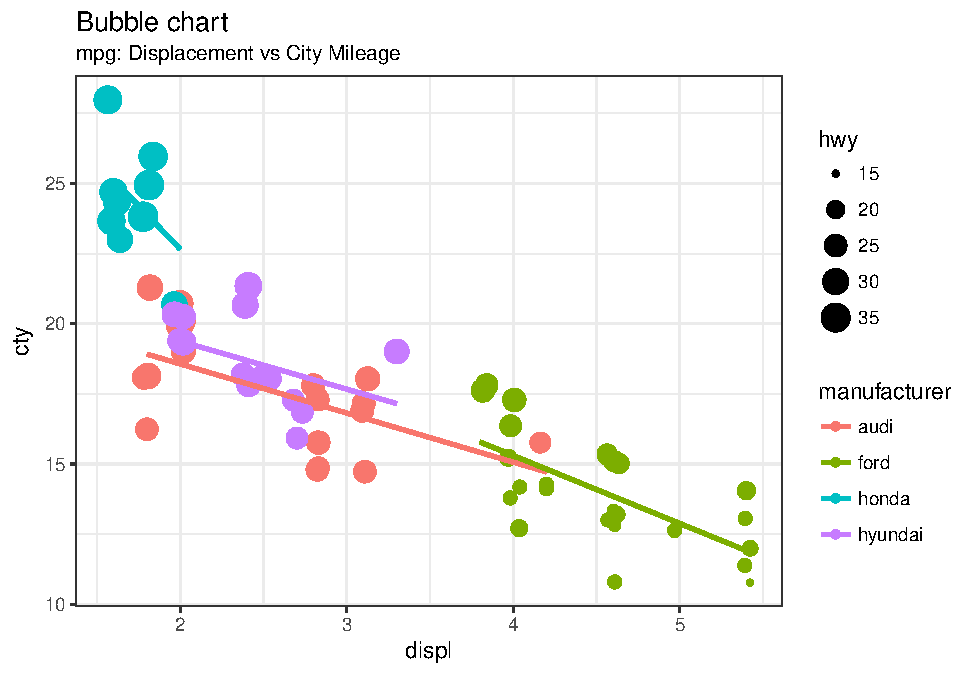
\includegraphics{class_0113_files/figure-latex/unnamed-chunk-7-1.pdf}

\section{12. facet을 이용해서 대륙별로 GDP와 기대수명에 대한 산점도를
그려보세요.}\label{facet---gdp----.}

\begin{Shaded}
\begin{Highlighting}[]
\NormalTok{a }\OperatorTok{+}\StringTok{ }\KeywordTok{facet_wrap}\NormalTok{(}\OperatorTok{~}\StringTok{ }\NormalTok{Continent)}
\end{Highlighting}
\end{Shaded}

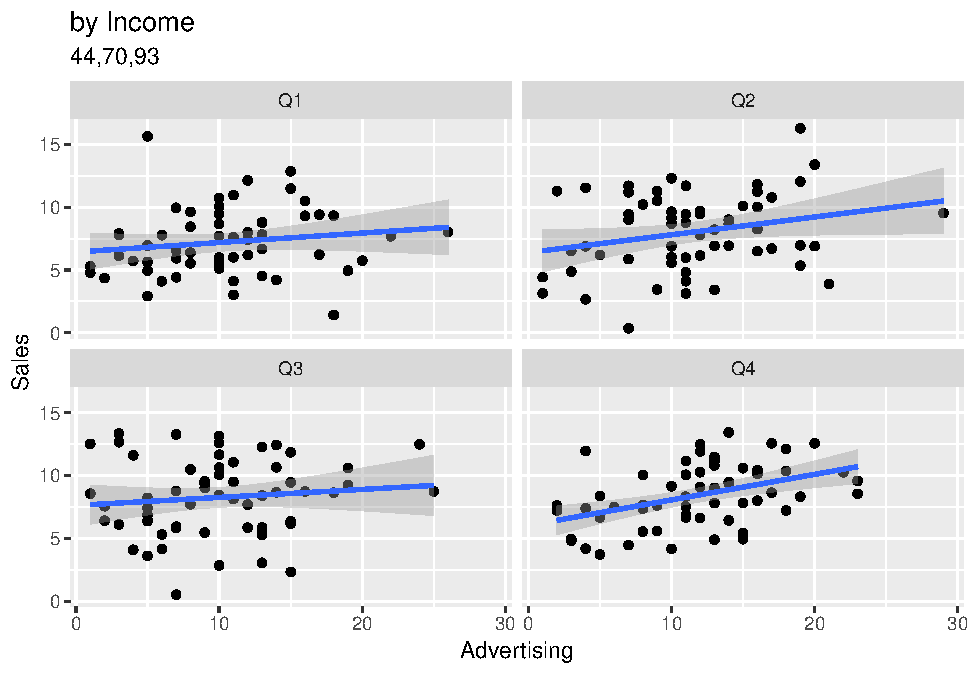
\includegraphics{class_0113_files/figure-latex/unnamed-chunk-8-1.pdf}

\section{13. 국가별로 성별에 따라 기대수명이 다릅니다. mutate함수를
사용해서 ageSexDiff라는 변수를 만들어
보세요.}\label{----.-mutate--agesexdiff---.}

\begin{Shaded}
\begin{Highlighting}[]
\NormalTok{dataset <-}\StringTok{ }\NormalTok{dataset }\OperatorTok\StringTok{ }\KeywordTok{mutate}\NormalTok{(}\DataTypeTok{ageSexDiff =}\NormalTok{ Female }\OperatorTok{-}\StringTok{ }\NormalTok{Male)}
\end{Highlighting}
\end{Shaded}

\section{14. 어떤 대륙에서 ageSexDiff가 가장 크고
작은가요?}\label{--agesexdiff---}

\begin{Shaded}
\begin{Highlighting}[]
\NormalTok{dataset }\OperatorTok\StringTok{ }
\StringTok{  }\KeywordTok{group_by}\NormalTok{(Continent) }\OperatorTok\StringTok{ }
\StringTok{  }\KeywordTok{summarise}\NormalTok{(}\DataTypeTok{contiSexDiff =} \KeywordTok{mean}\NormalTok{(ageSexDiff)) }\OperatorTok\StringTok{ }
\StringTok{  }\KeywordTok{arrange}\NormalTok{(}\KeywordTok{desc}\NormalTok{(contiSexDiff))}
\end{Highlighting}
\end{Shaded}

\begin{verbatim}
## # A tibble: 6 x 2
##   Continent     contiSexDiff
##   <chr>                <dbl>
## 1 Europe                6.00
## 2 South America         5.97
## 3 North America         5.52
## 4 Asia                  4.86
## 5 Oceania               4.71
## 6 Africa                3.72
\end{verbatim}

\section{15. 자유롭게 분석을 시작해보세요.}\label{--.}

\begin{Shaded}
\begin{Highlighting}[]
\CommentTok{# Dumbell plot (p25 in M24-ggplot2_Gallery)}
\KeywordTok{library}\NormalTok{(ggalt)}
\NormalTok{continentGender <-}\StringTok{ }\NormalTok{dataset }\OperatorTok\StringTok{ }
\StringTok{  }\KeywordTok{group_by}\NormalTok{(Continent) }\OperatorTok\StringTok{ }
\StringTok{  }\KeywordTok{summarise}\NormalTok{(}\DataTypeTok{avgMen =} \KeywordTok{mean}\NormalTok{(Male), }\DataTypeTok{avgWomen =} \KeywordTok{mean}\NormalTok{(Female)) }\OperatorTok\StringTok{ }
\StringTok{  }\KeywordTok{arrange}\NormalTok{(}\KeywordTok{desc}\NormalTok{(avgWomen))}
\NormalTok{b <-}\StringTok{ }\KeywordTok{ggplot}\NormalTok{(continentGender, }
            \KeywordTok{aes}\NormalTok{(}\DataTypeTok{x =}\NormalTok{ avgMen, }
                \DataTypeTok{xend =}\NormalTok{ avgWomen, }
                \DataTypeTok{y=} \KeywordTok{reorder}\NormalTok{(Continent, }\OperatorTok{-}\NormalTok{avgWomen), }
                \DataTypeTok{group =}\NormalTok{ Continent)) }\OperatorTok{+}
\StringTok{  }\KeywordTok{geom_dumbbell}\NormalTok{()}
\NormalTok{b}
\end{Highlighting}
\end{Shaded}

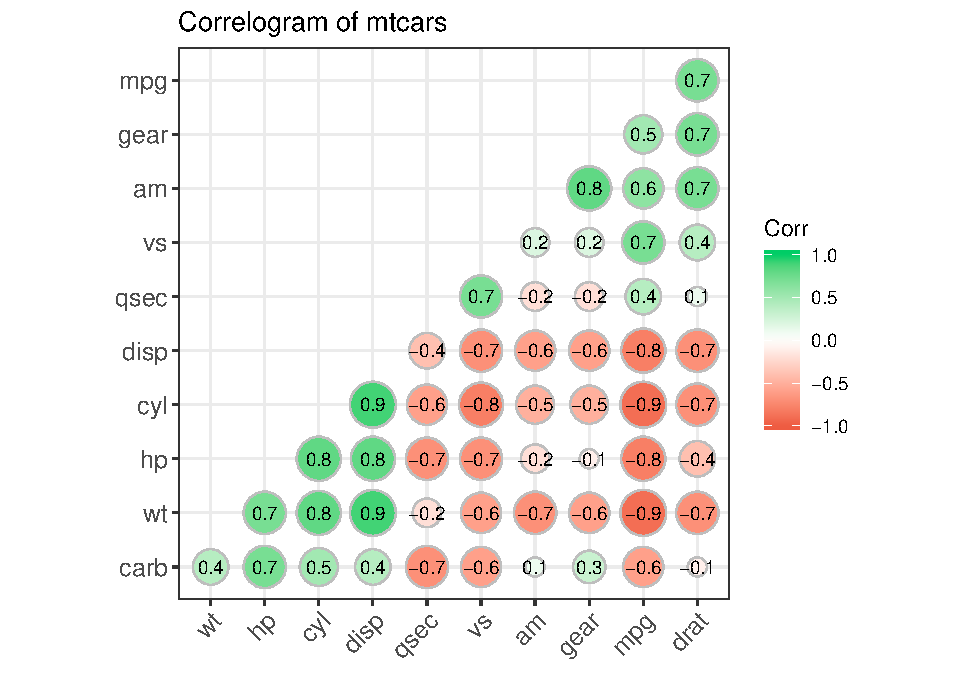
\includegraphics{class_0113_files/figure-latex/unnamed-chunk-11-1.pdf}

\begin{Shaded}
\begin{Highlighting}[]
\NormalTok{c <-}\StringTok{ }\NormalTok{b }\OperatorTok{+}\StringTok{ }
\StringTok{  }\KeywordTok{labs}\NormalTok{(}\DataTypeTok{x=}\OtherTok{NULL}\NormalTok{, }\DataTypeTok{y=}\OtherTok{NULL}\NormalTok{, }\DataTypeTok{title=}\StringTok{"Continents difference in life expectancy"}\NormalTok{,}
       \DataTypeTok{subtitle =} \StringTok{"left: Men, right: Women"}\NormalTok{,}
       \DataTypeTok{caption =} \StringTok{"Source: OECD"}\NormalTok{) }\OperatorTok{+}
\StringTok{  }\KeywordTok{theme}\NormalTok{(}\DataTypeTok{plot.title =} \KeywordTok{element_text}\NormalTok{(}\DataTypeTok{hjust=}\FloatTok{0.5}\NormalTok{, }\DataTypeTok{face=}\StringTok{"bold"}\NormalTok{),}
        \DataTypeTok{plot.background=}\KeywordTok{element_rect}\NormalTok{(}\DataTypeTok{fill=}\StringTok{"#f7f7f7"}\NormalTok{),}
        \DataTypeTok{panel.background=}\KeywordTok{element_rect}\NormalTok{(}\DataTypeTok{fill=}\StringTok{"#f7f7f7"}\NormalTok{),}
        \DataTypeTok{axis.ticks=}\KeywordTok{element_blank}\NormalTok{(),}
        \DataTypeTok{legend.position=}\StringTok{"top"}\NormalTok{,}
        \DataTypeTok{panel.border=}\KeywordTok{element_blank}\NormalTok{())}
\NormalTok{c}
\end{Highlighting}
\end{Shaded}

\includegraphics{class_0113_files/figure-latex/unnamed-chunk-11-2.pdf}

\section{\texorpdfstring{18. \texttt{classProject1.R}을 저장해서
\href{mailto:learningSpoonsR@gmail.com}{\nolinkurl{learningSpoonsR@gmail.com}}
로
보내주세요.}{18. classProject1.R을 저장해서 learningSpoonsR@gmail.com 로 보내주세요.}}\label{classproject1.r--learningspoonsrgmail.com--.}


\end{document}
